\documentclass[tikz]{standalone}
\usepackage{pgfplots}
\pgfplotsset{compat=1.15}
\usepackage{mathrsfs}
\usetikzlibrary{arrows,calc}
\usepackage{tkz-euclide}
\pagestyle{empty}

\definecolor{AngleClr}{rgb}{0,0.39215686274509803,0}
\definecolor{ShapeClr}{rgb}{0.6,0.2,0}

\begin{document}

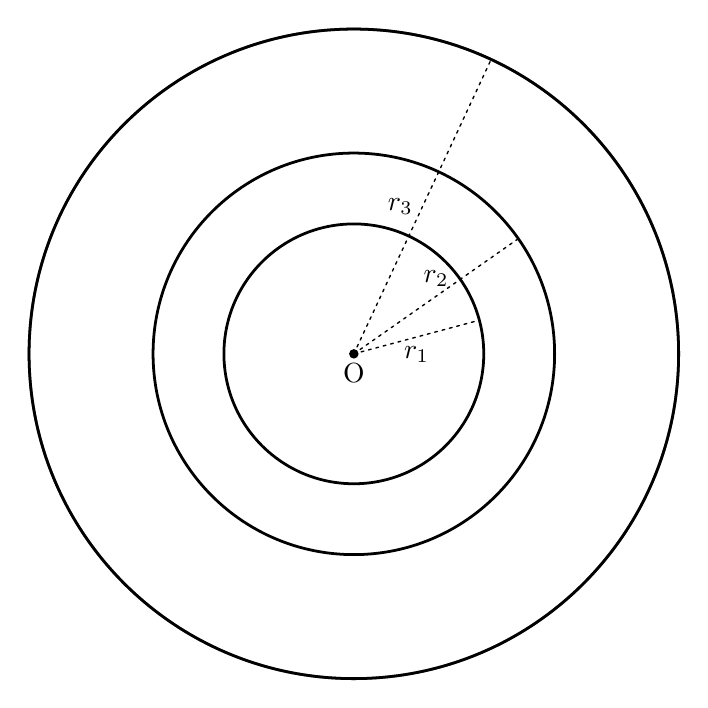
\begin{tikzpicture}[scale=.75]
\tkzSetUpLine[line width=1pt,color=black]
\tkzSetUpPoint[fill=black]

\tkzDefPoints{0/0/O,2.2/0/A,3.4/0/B,5.5/0/C}

\tkzDefPoint(15:2.2){AA}
\tkzDefPoint(35:3.4){BB}
\tkzDefPoint(65:5.5){CC}

\tkzDrawCircle[line width=1.0pt,fill=white](O,C)

\tkzDrawSegments[line width=0.5pt,color=black,dashed,dash pattern=on 1pt off 1.75pt](O,AA O,BB O,CC)

\tkzDrawCircle[line width=1.0pt,color=black](O,A)
\tkzDrawCircle[line width=1.0pt,color=black](O,B)
\tkzDrawCircle[line width=1.0pt,color=black](O,C)

\tkzLabelSegment(O,AA){$r_1$}
\tkzLabelSegment[above](O,BB){$r_2$}
\tkzLabelSegment[left](O,CC){$r_3$}


\tkzDrawPoints[size=3](O)
\tkzLabelPoint[below](O){$\rm O$}



\end{tikzpicture}
\end{document}
